\documentclass[10pt]{article}
\usepackage[a4paper,bottom=3cm]{geometry}
\usepackage[english]{babel}
\usepackage[utf8]{inputenc}
\usepackage{amsmath}
\usepackage{amsthm}
\usepackage{amssymb}
\usepackage{graphicx}
\usepackage{subfig}
\usepackage{hyperref}

\theoremstyle{definition}
\newtheorem{definition}{Definition}[section]

\author{Julian Bopp, Takudzwa Togarepi}
\title{Sex and stature prediction from partial femurs using statistical shape modelling}
\begin{document}

\maketitle

\begin{abstract}
\noindent
Due to the femur bone's sheer size and strength, it holds immense significance within the human anatomy especially within the field of forensic science. Upon careful analysis, the femur bone offers invaluable insights into the identification of an individual's gender, stature and even geographic origin. This is due to the fact that femurs of individuals who are of the same geographic origin, gender and similar stature have similar femur bones. However, it is not unusual to come across incomplete or distorted femurs during the examination of human remains. This could be as result of death by accidents or other factors. This leads to a rise in the need for femur reconstruction, which in turn allows the modelling of complete femur structure and facilitates in-depth analysis. In an attempt to address this need, our project aims to  provide a model to effectively reconstruct partial femurs and use them to predict the gender and the stature of whoever the femurs belonged to.\\

\noindent
$\bold{Keywords}$: femur, forensics, identification, gender prediction, reconstruction, modeling, stature.\\

\end{abstract}
\section{Introduction} From a set of given femur data we train a regression model to predict sex and stature.
We then use Bayesian model fitting techniques to be able reconstruct a complete bone from a partial femur. This means that we find the parameters of the shape model that best describe the partial bone. Given this reconstruction we can aquire the necessary measurements of the bone to use our regression model to predict the sex and stature from a partial bone.

\section{Methods}
We introduce the problem setting and list the methods used to solve it.

\begin{definition}[Bayesian linear regression]
We assume that a variable $y$ is modelled as a linear function of $x$. More precisely our assumption is
\begin{equation}
y \sim N(a\cdot x + b, \sigma^2).
\end{equation}
Let $\theta = (a,b,\sigma^2)$. Given $X=(x_1,\dots,x_n)$ and $Y=(y_1,\dots,y_n)$, we want to estimate $\theta$ using the posterior
$$p(\theta|X,Y) \propto p(Y|\theta,X)p(\theta).$$
\end{definition}

\noindent
The way we solve the Bayesian regression model in scalismo is by specifying priors over the parameters and using the Metropolis Hastings algorithm. The Metropolis Hastings algorithm allows us to iteratively draw samples from the posterior distribution.

\begin{definition}[Metropolis Hastings Algorithm]\label{def:metro}
Given an initial sample $x$ and a proposal distribution $Q$ that is used to propose new samples we do the following steps:
\begin{enumerate}
\item Draw a sample $x'$ from $Q(x'|x)$.
\item With probability $$\alpha=\text{min}\{\frac{p(x')Q(x|x')}{p(x)Q(x'|x)},1\}$$
accept $x'$ as new state $x$.
\item Emit current state $x$ as sample
\end{enumerate}
\end{definition}

\noindent
The Scalismo library provides us with the tools to easily sample a posterior distribution using the Metropolis Hastings Algorithm. As seen in the PSM-Fitting Course we can treat the Shape model fitting problem as Bayesian linear regression, therefore we can use the Metropolis Hastings Algorithm to fit shapes.



\section{Experiments and results}

\subsection{Data and experimental setup}
In this experiment, two datasets are used. One consists of a table of 42 measurements of stature, femur-bone-length, trochanter-distance and sex of a person. An excerpt of this data can be seen in table \ref{table:1}.

\begin{table}[h]
    \centering
    \begin{tabular}{l|l|l|l|l}
        id & sex & stature & bone-length & trochanter-distance \\ \hline
        rmi-femur-0 & f & 1580.0 & 383.3406419563092 & 58.555946364648 \\ \hline
        rmi-femur-1 & f & 1780.0 & 416.12659236042094 & 70.14034429582061 \\ \hline
        rmi-femur-10 & m & 1800.0 & 456.1085369397006 & 63.598123395135545 \\ \hline
        rmi-femur-11 & m & 1900.0 & 452.1018813239008 & 68.02134385658242 \\ \hline
        rmi-femur-12 & m & 1840.0 & 450.85399522717535 & 76.27473182565058 \\ \hline
        rmi-femur-13 & f & 1700.0 & 427.2560495653345 & 64.53255033056375 \\
    \end{tabular}
    \caption{6 entries from the real world femur measurement dataset.}
    \label{table:1}
\end{table}

\noindent
The second data set consists of 10 3D partial femurs meshes. Some partial femurs are almost a complete bone, like in figure \ref{fig:1}, and in others almost the complete bone is missing, like in figure \ref{fig:2}.

\begin{figure}[h]
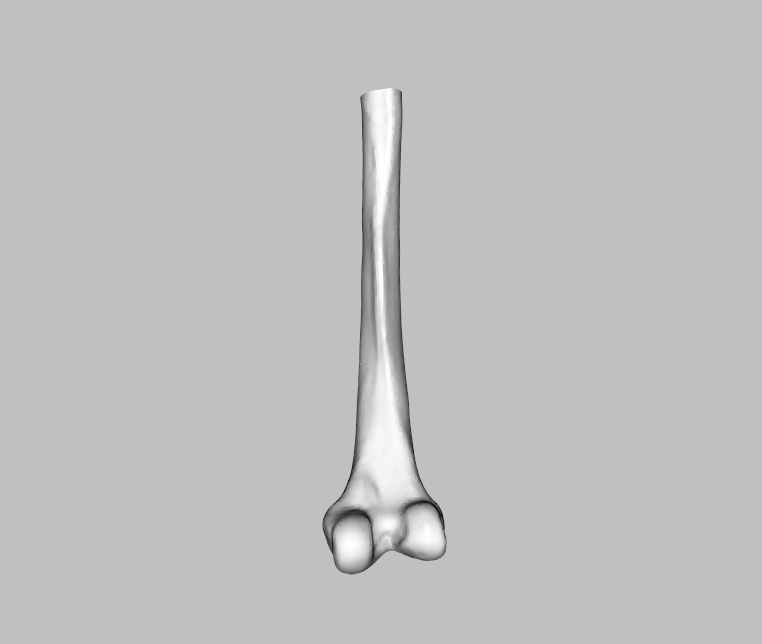
\includegraphics[scale=0.3]{partial1.png}
\centering
\caption{Partial femur with head missing.}
\label{fig:1}
\end{figure}

\begin{figure}[h]
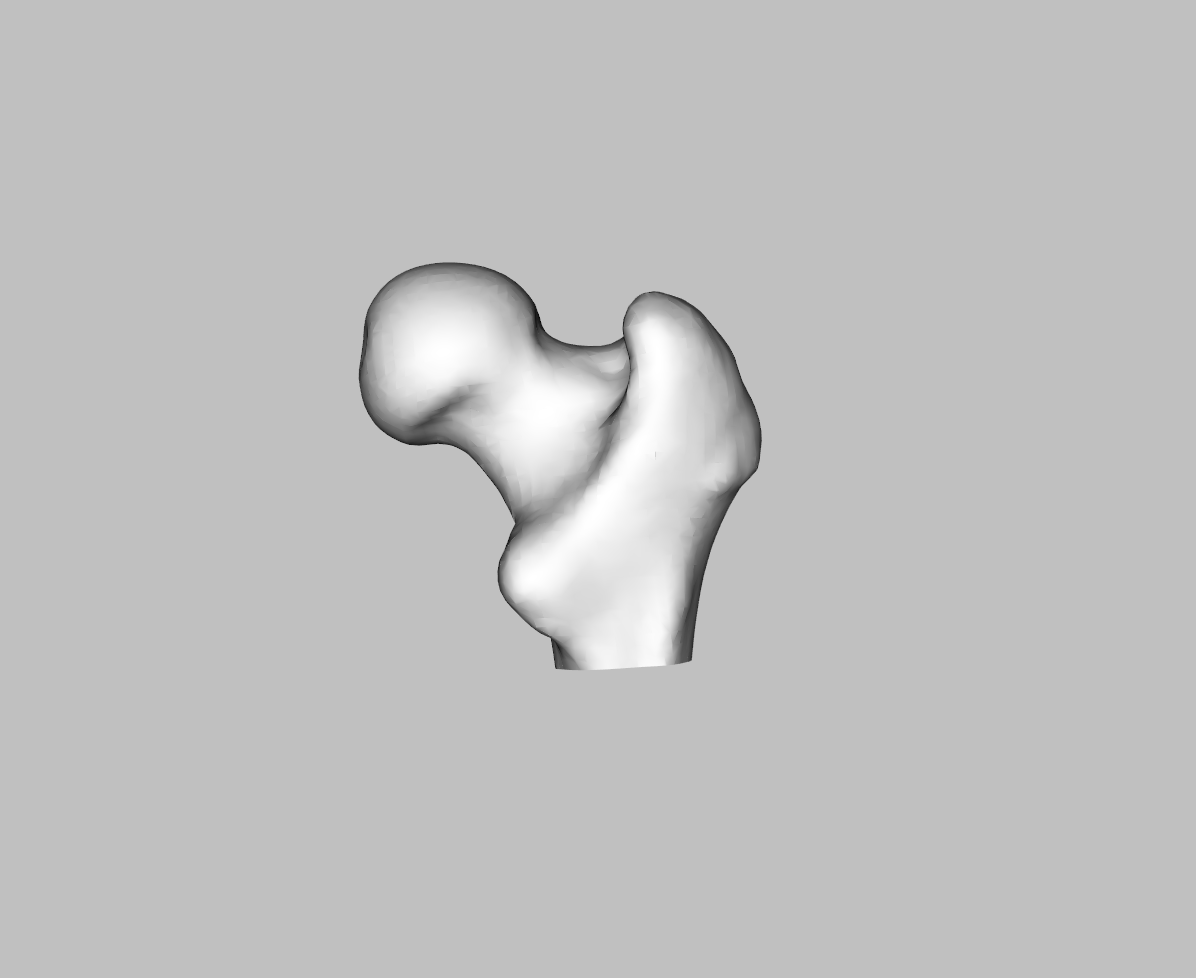
\includegraphics[scale=0.2]{partial2.png}
\centering
\caption{Partial femur with nothing but a head.}
\label{fig:2}
\end{figure}

\noindent
We first train a linear and logistic regression model using the metropolis hastings algorithm \ref{def:metro}, on the the measurements from the table. We confirm our regression with posterior predictive checks.

\begin{figure}[h!]
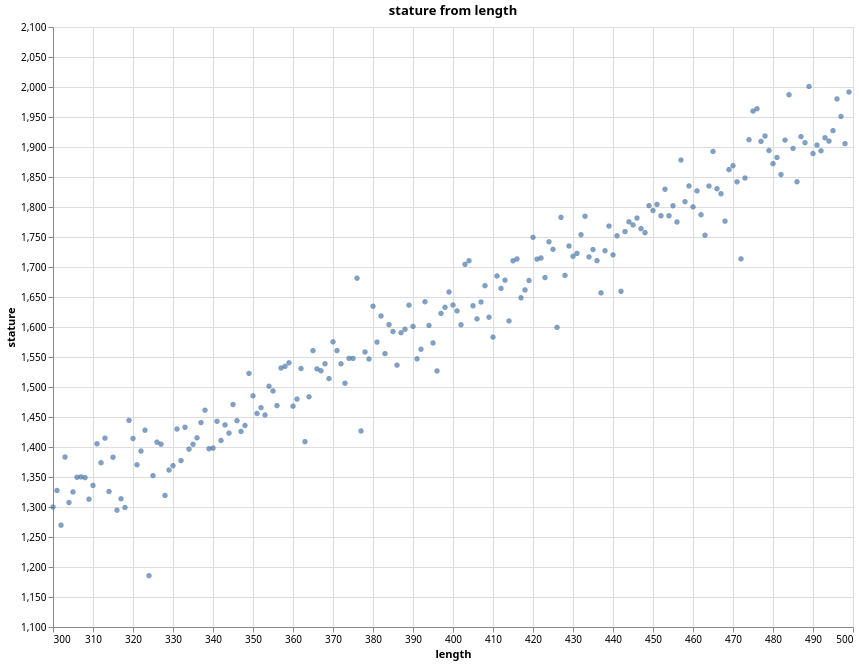
\includegraphics[scale=0.4]{ppc_linear_scatter.png}
\centering
\caption{Posterior predictive check for linear regression model predicting stature from femur length.}
\label{fig:3}
\end{figure}

\begin{figure}[h!]
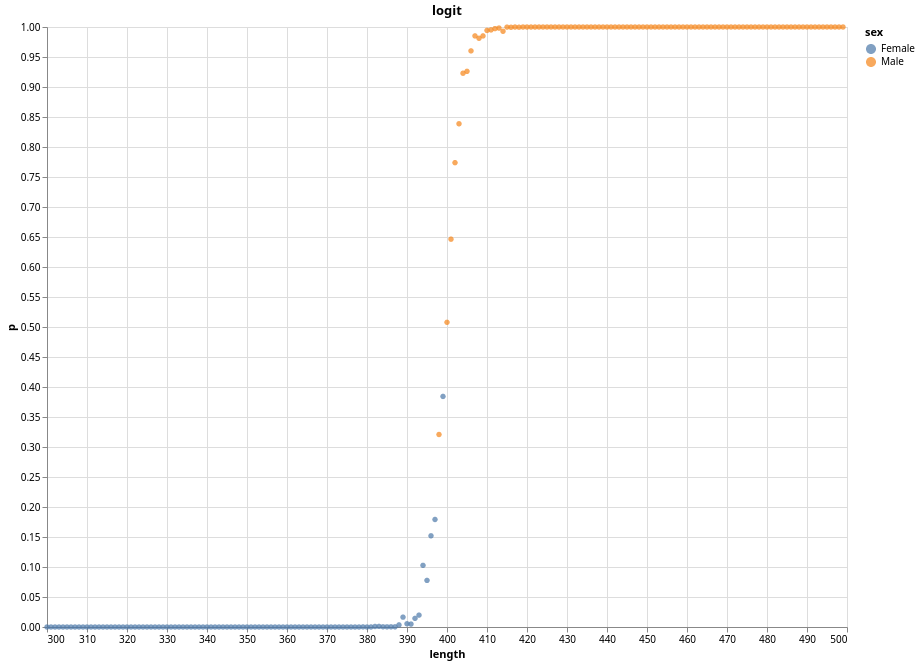
\includegraphics[scale=0.4]{ppc_logistic_scatter.png}
\centering
\caption{Posterior predictive check for logistic regression model predicting sex from femur length.}
\label{fig:4}
\end{figure}
\noindent
Afterwards we fit the partial femurs to our model. For this we used a mixture approach with Gaussian random walk proposals.
We then take the length measurements from the fitted model and use our regression model to predict their sex and stature.

\subsection{Experimental results}
We present the length measurements from the reconstructed femurs, and the estimated stature and sex, in table \ref{table:2}.

\begin{table}[h!]
    \centering
    \begin{tabular}{l|l|l|l}
        id & bone-length & stature & sex \\ \hline
        0 & 393  & 1603 & f \\ \hline
        1 & 442  & 1758 & m \\ \hline
        2 &  439 & 1748 & m \\ \hline
        3 &  425 & 1703 & m \\ \hline
        4 &  430 & 1719 & f \\ \hline
        5 &  429 & 1718 & f \\ \hline
        6 &  442 & 1759 & m \\ \hline
        7 &  440 & 1758 & m \\ \hline
        8 &  427 & 1711 & f \\ \hline
        9 &  476 & 1865 & m \\

    \end{tabular}
    \caption{Length measurements from reconstructed femurs}
    \label{table:2}
\end{table}

\begin{figure}[h!]
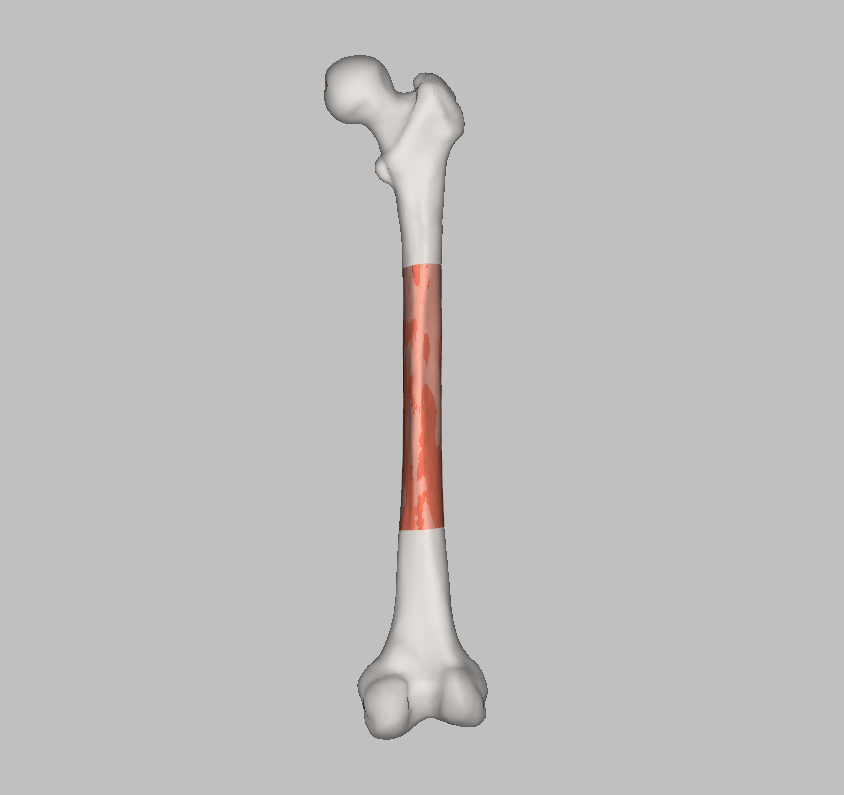
\includegraphics[scale=0.3]{fit1.png}
\centering
\caption{Model fit to partial bone}
\label{fig:5}
\end{figure}

We can see in figure \ref{fig:4} that the model fits the bone rather well. Furthermore we plot the trace plot of the log likelihood values in figure \ref{fig:5}.
\begin{figure}[h!]
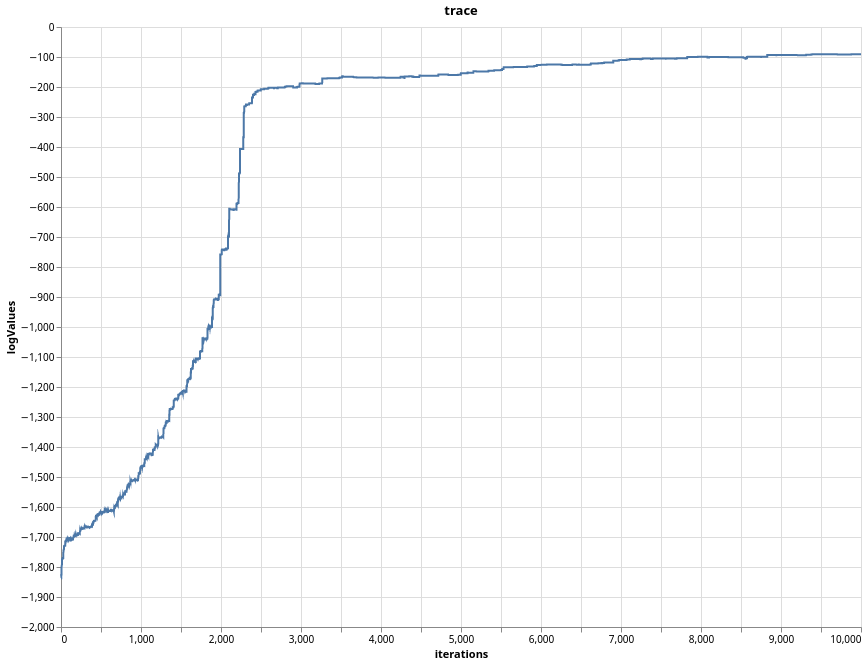
\includegraphics[scale=0.4]{trace8.png}
\centering
\caption{Model fit to partial bone}
\label{fig:6}
\end{figure}
\newpage
\section{Conclusion}

We constructed a method to estimate the sex and stature of a person with only the knowledge of a partial femur bone. What we we were not able to do is quantifying the uncertainty of our estimate. This is a very important task that is left to do.

There are many parameters that need fine tuning in the pipeline used in the Metropolis Hastings algorithm. Due to time constraints we were certainly not able to choose the optimal parameters, or even come close to the optimal parameters. Further testing and validating would only result in improving the model furher further.

\noindent
From the trace plit in figure \ref{fig:6} we conclude that the Metropolis Hastings algorithm gets stuck in a local maxima. Further tuning is necessary to escape this maxima and explore the whole space better.

\end{document}
